\section{Biometria}\label{sec:biometria}

Realizando a composição dos termos gregos “bio”, que significa vida, e “metria”, que
significa medida, forma-se a palavra biometria, que é um ramo da ciência que busca
identificar ou verificar a identidade de uma pessoa baseado nas suas características
físicas ou comportamentais \cite{refer6}. As características físicas, como
impressão digital, face e íris, medem a estrutura ou a forma de uma parte específica do
corpo de uma pessoa, enquanto que as características comportamentais estão mais
preocupadas em como uma pessoa faz devida ação, como por exemplo, falar \cite{refer7}.

A autenticação biométrica é um processo que permite determinar a identidade de um
indivíduo tomando como base quem ele é ao invés de algo que ele lembra ou possui.
Dependendo do contexto em que for utilizada a autenticação biométrica pode operar de
duas formas diferentes: verificação e identificação \cite{refer6}.


Independente da característica a ser utilizada para realizar a autenticação
biométrica, seja ela física ou comportamental, algumas propriedades devem ser
elencadas para que uma medida biométrica seja considerada útil, que são \cite{refer8}:
a) universalidade: todo indivíduo deve possuir a medida em questão;
b) unicidade: ser suficientemente diferente entre os indivíduos;
c) inalterabilidade: se manter estável em função do tempo;
d) mensurabilidade: ser passível de captura e digitalização;
e) aceitabilidade: os indivíduos devem concordar em fornecer a medida biométrica.

Apesar de não ser o meio com a melhor unicidade e mais segura, por ser um processo de fácil utilização prática, menos invasiva o reconhecimento facial foi escolido. Os outros modos de medidas biométricas apesar de oferecerem mais vantagens não oferecem a praticidade e viabilidade que é demandada pelo requisito da aplicação.

\begin{figure}[ht]
\centering
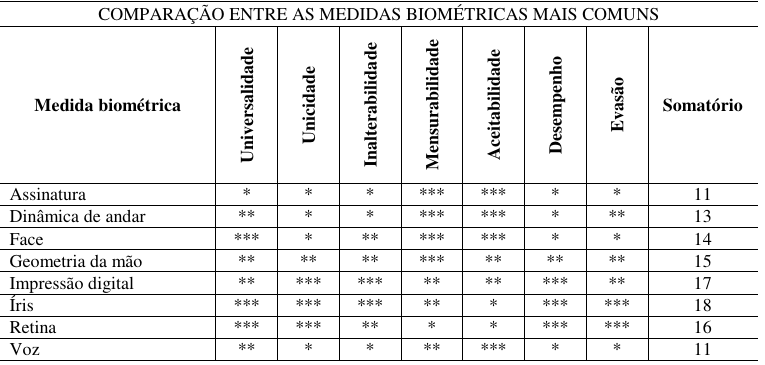
\includegraphics[width=8cm]{images/comparacao.png}
\caption{Comparação entre as medidas biométricas mais comuns. }
\label{fig:comparacao}
\end{figure}
